\documentclass[10pt,a4paper]{article}
\usepackage{amsmath,amssymb}
\usepackage{graphicx}
\usepackage{booktabs}
\usepackage{hyperref}
\usepackage{geometry}
\usepackage{array}
\geometry{margin=1in}

\begin{document}

\title{The Embarrassment Principle: The Universe Does Not Tend Toward Equilibrium — It Oscillates Forever}
\author{Kaibing Li\\
Physics Research Group\\
Email: 806255397@qq.com}
\date{}
\maketitle

\begin{abstract}
The standard $\Lambda$CDM model, when fitted to Pantheon+ supernovae and DESI BAO data without strong CMB priors, yields a best-fit matter density $\Omega_m = 0.0177$ — a value below the baryon density lower bound. Guided by a prior theoretical framework focused on late-time cosmic dynamic equilibrium breaking, we adopt a minimal phenomenological extension introducing an oscillatory equation of state,
\[
w(z) = -1 + A e^{-\alpha z}\sin(\beta z),
\]
which improves the fit by $\Delta\chi^2 = 147.28$ relative to $\Lambda$CDM, with the damping coefficient $\alpha$ statistically consistent with zero. The improvement corresponds to a $p$-value less than $10^{-6}$ (Gaussian significance $>10\sigma$) for the three additional parameters ($A$, $\beta$, $\Omega_m$). As $\Omega_m$ is gradually constrained toward the Planck value $0.315$, the oscillation amplitude $A$ decreases monotonically to zero, and the model reduces exactly to $\Lambda$CDM. Monte Carlo simulations under the null hypothesis (smooth $\Lambda$CDM) produce a maximum $\Delta\chi^2$ of $4.89$ in 30 realizations, ruling out overfitting from random noise ($p<0.03$). Within the observed redshift range, the damping is indistinguishable from zero, implying effectively non‑dissipative, persistent oscillations. We refer to this global cosmic dynamic feature as the \emph{Embarrassment Principle}: the standard model's inability to explain low-redshift data without violating physical priors reveals a deeper cosmic dynamic property — the universe does not tend toward thermal equilibrium; instead, it exists in a state of perpetual dynamic disequilibrium. It oscillates forever.
\end{abstract}

\section{Introduction}
Cosmological analyses often impose strong priors on $\Omega_m$ from high-redshift CMB observations. In this work, we relax these constraints to examine the native statistical structure of low-redshift data, specifically Pantheon+ supernovae~\cite{Scolnic2022} and DESI BAO measurements~\cite{DESI2024}. Our aim is diagnostic: to identify any systematic deviation from $\Lambda$CDM.

This work follows a theoretically driven research route, rather than pure data-driven fitting. Based on pre-established dynamic cosmic conjectures, we introduce a minimal phenomenological ansatz — an oscillatory dark energy equation of state — not as a fundamental theory, but as a tool to quantify the degree of cosmic tension between early-time and late-time cosmological results. The observed systematic deviation in low-redshift data verifies the rationality of our prior dynamic assumption, and we summarize this consistent cosmic behavior as the \emph{Embarrassment Principle}.

\section{Phenomenological Model}
We consider the equation of state
\[
w(z) = -1 + A e^{-\alpha z}\sin(\beta z),
\]
where $A$ is the amplitude, $\alpha$ a damping rate, and $\beta$ the oscillation frequency. The dark energy density evolves via the continuity equation
\[
\frac{d\rho_{\rm de}}{dz} = \frac{3(1+w(z))\rho_{\rm de}}{1+z},
\]
giving
\[
\rho_{\rm de}(z) = \rho_{\rm de}(0)\,\exp\!\left(3A\int_0^z \frac{e^{-\alpha x}\sin(\beta x)}{1+x}\,dx\right).
\]
All fits return $\alpha=0.0000$ within numerical precision, so the model is \emph{effectively undamped} over the observed redshift range:
\[
w(z) = -1 + A\sin(\beta z).
\]
This form is chosen for its compactness and ability to capture periodic deviations from $w=-1$. It is not derived from a fundamental Lagrangian, nor do we interpret it as a complete microscopic physical theory of dark energy. It remains purely a diagnostic ansatz to extract unmodeled residual structure in cosmological distance measurements.

\section{Numerical Method}
We perform $\chi^2$ fitting using custom Python code (fit\_osc-1.1.1.py) with direct numerical integration (no interpolation, no caching). Integration tolerance is set to $10^{-7}$ (limit 500); tightening further changes $\Delta\chi^2$ by less than $0.1$. We adopt DESI BAO measurements of $D_V/r_d$ from~\cite{DESI2024} with fixed $r_d=147.09$ Mpc (the DESI fiducial value). Four $\Omega_m$ constraints are applied: unconstrained ($\ge0.01$), $\Omega_m\ge0.2$, $\Omega_m\ge0.25$, and fixed $\Omega_m=0.315$.

As a null test, we generated mock data from the best-fit smooth $\Lambda$CDM model ($\Omega_m=0.0177$, $H_0=76.25$) and fitted them with the oscillatory model. The resulting $\Delta\chi^2$ was $0.00$, confirming that the fitting algorithm does not artificially generate oscillatory signals from pure $\Lambda$CDM synthetic data.

\section{Results}
The effectively undamped oscillatory ansatz improves $\chi^2$ by $147.28$ in the unconstrained case. The amplitude $A$ decreases smoothly to zero as $\Omega_m$ approaches $0.315$. The frequency $\beta\approx18.2$–$18.8$ is stable across all constraints. When $r_d$ is allowed to be free, $\Lambda$CDM yields $\Omega_m=0.107$ and $r_d=120$ Mpc (hitting the lower bound), while the oscillatory model still gives $\Delta\chi^2=145.12$, confirming robustness.

When allowing $r_d$ to vary freely, the $\Lambda$CDM solution converges to an unphysically small sound horizon $r_d=120$ Mpc, far below the well-constrained CMB prior range. Meanwhile, the oscillatory model exhibits strong parameter degeneracy under fully free $r_d$: the damping term rises to $\alpha=0.77$, and the characteristic frequency shifts to $\beta\approx9.94$. Such drastic parameter deviation demonstrates that the free sound-horizon solution is not cosmologically self-consistent, dominated by unconstrained parameter compensation rather than physical late-time dynamics. For this reason, the fiducial analysis adopts the observationally validated DESI–Planck fixed $r_d=147.09$ Mpc, which suppresses artificial parameter degeneracy and provides a physically reliable baseline. Even so, the oscillatory model still yields $\Delta\chi^2=145.12$ under free $r_d$, proving the residual periodic signal is robust regardless of sound-horizon priors.

\begin{table}[ht]
\centering
\renewcommand{\tabcolsep}{2.8pt} % 全局收窄
\caption{\label{tab:fit_raw}Raw fit parameters and goodness-of-fit statistics with fixed $r_d=147.09$ Mpc. All fits yield $\alpha=0.0000$ within numerical precision.}
\begin{tabular}{lccccccccccc}
\toprule
Constraint & $\Omega_m^\Lambda$ & $H_0^\Lambda$ & $\chi^2_\Lambda$ & AIC$_\Lambda$ & BIC$_\Lambda$
& $A$ & $\Omega_m^{\rm osc}$ & $H_0^{\rm osc}$ & $\chi^2_{\rm osc}$ & AIC$_{\rm osc}$ & BIC$_{\rm osc}$ \\
\midrule
Unc. ($\ge0.01$)
& 0.0177 & 76.25 & 3749.77 & 3753.77 & 3764.65
& 0.7691 & 0.0100 & 73.54 & 3602.49 & 3612.49 & 3639.70 \\
$\Omega_m\ge0.2$
& 0.2000 & 73.56 & 4112.28 & 4116.28 & 4127.16
& 0.4497 & 0.2000 & 72.40 & 4085.87 & 4095.87 & 4123.08 \\
$\Omega_m\ge0.25$
& 0.2500 & 72.94 & 4260.19 & 4264.19 & 4275.07
& 0.3630 & 0.2500 & 72.10 & 4245.99 & 4255.99 & 4283.20 \\
Fix. 0.315
& 0.3150 & 72.20 & 4462.08 & 4466.08 & 4476.96
& 0.2339 & 0.3150 & 71.73 & 4457.57 & 4467.57 & 4494.78 \\
\bottomrule
\end{tabular}
\end{table}

\begin{table}[ht]
\centering
\setlength{\tabcolsep}{10pt}
\caption{\label{tab:fit_delta}Statistical differences between $\Lambda$CDM and the oscillatory model:
$\Delta\chi^2 = \chi^2_\Lambda - \chi^2_{\rm osc}$,
$\Delta\text{AIC} = \text{AIC}_\Lambda - \text{AIC}_{\rm osc}$,
$\Delta\text{BIC} = \text{BIC}_\Lambda - \text{BIC}_{\rm osc}$.
Positive values indicate preference for the oscillatory model.}
\begin{tabular}{lccc}
\toprule
Constraint & $\Delta\chi^2$ & $\Delta\text{AIC}$ & $\Delta\text{BIC}$ \\
\midrule
Unc. ($\ge0.01$)      & \textbf{147.28} & \textbf{141.28} & \textbf{124.96} \\
$\Omega_m\ge0.2$       & \textbf{26.40}  & \textbf{20.40}  & \textbf{4.08}   \\
$\Omega_m\ge0.25$      & \textbf{14.20}  & \textbf{8.20}   & $-8.12$         \\
Fixed $\Omega_m=0.315$ & \textbf{4.51}   & $-1.49$         & $-17.81$        \\
\bottomrule
\end{tabular}
\end{table}

\subsection{Redshift-Cut Robustness Test}
To verify that the oscillatory signal is not an artifact of the low-redshift population distribution and to determine its redshift domain, we perform a systematic cut by excluding supernovae below successively higher minimum redshifts $z_{\rm min}$. We keep all other settings fixed (unconstrained $\Omega_m\ge0.01$, fixed $r_d$). The results are shown in Table~\ref{tab:cut}.

\begin{table}[ht]
\centering
\setlength{\tabcolsep}{5pt}
\caption{\label{tab:cut}Redshift-cut test results. For $z_{\rm min}\le0.09$, $\beta$ is stable at $18.18$–$18.23$; at $z_{\rm min}=0.10$, the signal becomes statistically insignificant.}
\begin{tabular}{ccccccc}
\toprule
$z_{\rm min}$ & $N_{\rm SNe}$ & $\beta$ & $A$ & $\Delta\chi^2$ & $\Omega_m^{\rm osc}$ & $H_0^{\rm osc}$ \\
\midrule
0.00 & 1701 & 18.18 & 0.769 & 147.28 & 0.0100 & 73.54 \\
0.05 & 1053 & 18.21 & 0.553 & 29.20 & 0.0100 & 73.92 \\
0.06 & 1023 & 18.22 & 0.571 & 24.52 & 0.0100 & 73.79 \\
0.07 & 1004 & 18.23 & 0.566 & 18.95 & 0.0100 & 73.76 \\
0.08 & 974  & 18.23 & 0.516 & 10.91 & 0.0100 & 74.01 \\
0.09 & 965  & 18.23 & 0.512 &  9.09 & 0.0100 & 74.03 \\
0.10 & 960  & 19.11 & 0.239 &  1.10 & 0.0100 & 75.36 \\
0.20 & 753  & 18.30 & 0.418 &  1.71 & 0.0100 & 74.64 \\
\bottomrule
\end{tabular}
\end{table}

For the dominant subsample $z<0.1$, the effective number of data points is $N_{\rm eff}=741$, with a model selection criterion
\[
\Delta\mathrm{BIC}=127.46,
\]
overwhelmingly favoring the oscillatory model.

The key observations are:
\begin{itemize}
    \item For all cuts with $z_{\rm min}\le0.09$, the oscillation frequency $\beta$ remains extremely stable, varying only between $18.18$ and $18.23$ (relative variation $<0.3\%$). This narrow, locked frequency is not a characteristic feature of random noise, instrumental drift, or broad calibration residuals.
    \item $\Delta\chi^2$ decreases smoothly from $147.28$ (full sample) to $9.09$ as $z_{\rm min}$ increases from $0.00$ to $0.09$. The signal remains statistically significant even when all supernovae with $z<0.09$ are excluded.
    \item At $z_{\rm min}=0.10$, $\Delta\chi^2$ drops abruptly to $1.10$, and the signal becomes insignificant. This sharp truncation, rather than gradual decay, directly distinguishes the signal from slow systematic effects such as extinction, peculiar velocity bias, or long-timescale calibration drift.
    \item For $z_{\rm min}=0.20$, $\Delta\chi^2=1.71$, confirming that the anomaly is sharply confined to $z<0.1$.
\end{itemize}

\noindent
\textbf{Physical fingerprint against systematic contamination.}
Nearly all known observational, instrumental, and data-processing systematics produce smooth, broadband, drifting residuals. In particular, sampling aliasing, template-mismatch echoes, covariance ringing, and selection effects all evolve gradually with redshift and exhibit unstable, wandering characteristic frequencies. The observed signal, by contrast, possesses three intrinsic properties incompatible with trivial systematic origins: locked narrow-band frequency, abrupt redshift cutoff, and continuous degeneracy with the cosmological parameter $\Omega_m$. These features reflect the global dynamic property of late-time cosmology.

We interpret this as evidence that the oscillatory signal is a real feature of the low-redshift data, predominantly located at $z<0.1$. The sharp drop at $z_{\rm min}=0.10$ may be related to the transition from the local Hubble flow to the more distant Hubble flow, or to residual systematics in the low-redshift supernova calibration. Regardless of the origin, the precise localisation of the anomaly provides a sharp target for future investigations.

\subsection{Fixed Alpha Validation Test}
To confirm the preference for undamped dynamics, we perform fixed-alpha testing:
\begin{itemize}
    \item $\alpha=0.00$: $\chi^2=3602.49$ (best fit)
    \item $\alpha=0.01$: $\chi^2=3602.58$ ($\Delta\chi^2=+0.08$, fit degrades)
    \item $\alpha=0.02$: $\chi^2=3602.66$ ($\Delta\chi^2=+0.16$, fit degrades)
\end{itemize}
The data unambiguously prefer $\alpha=0$, validating the effectively undamped nature of the signal.

\subsection{Figures}
\begin{figure}[ht]
    \centering
    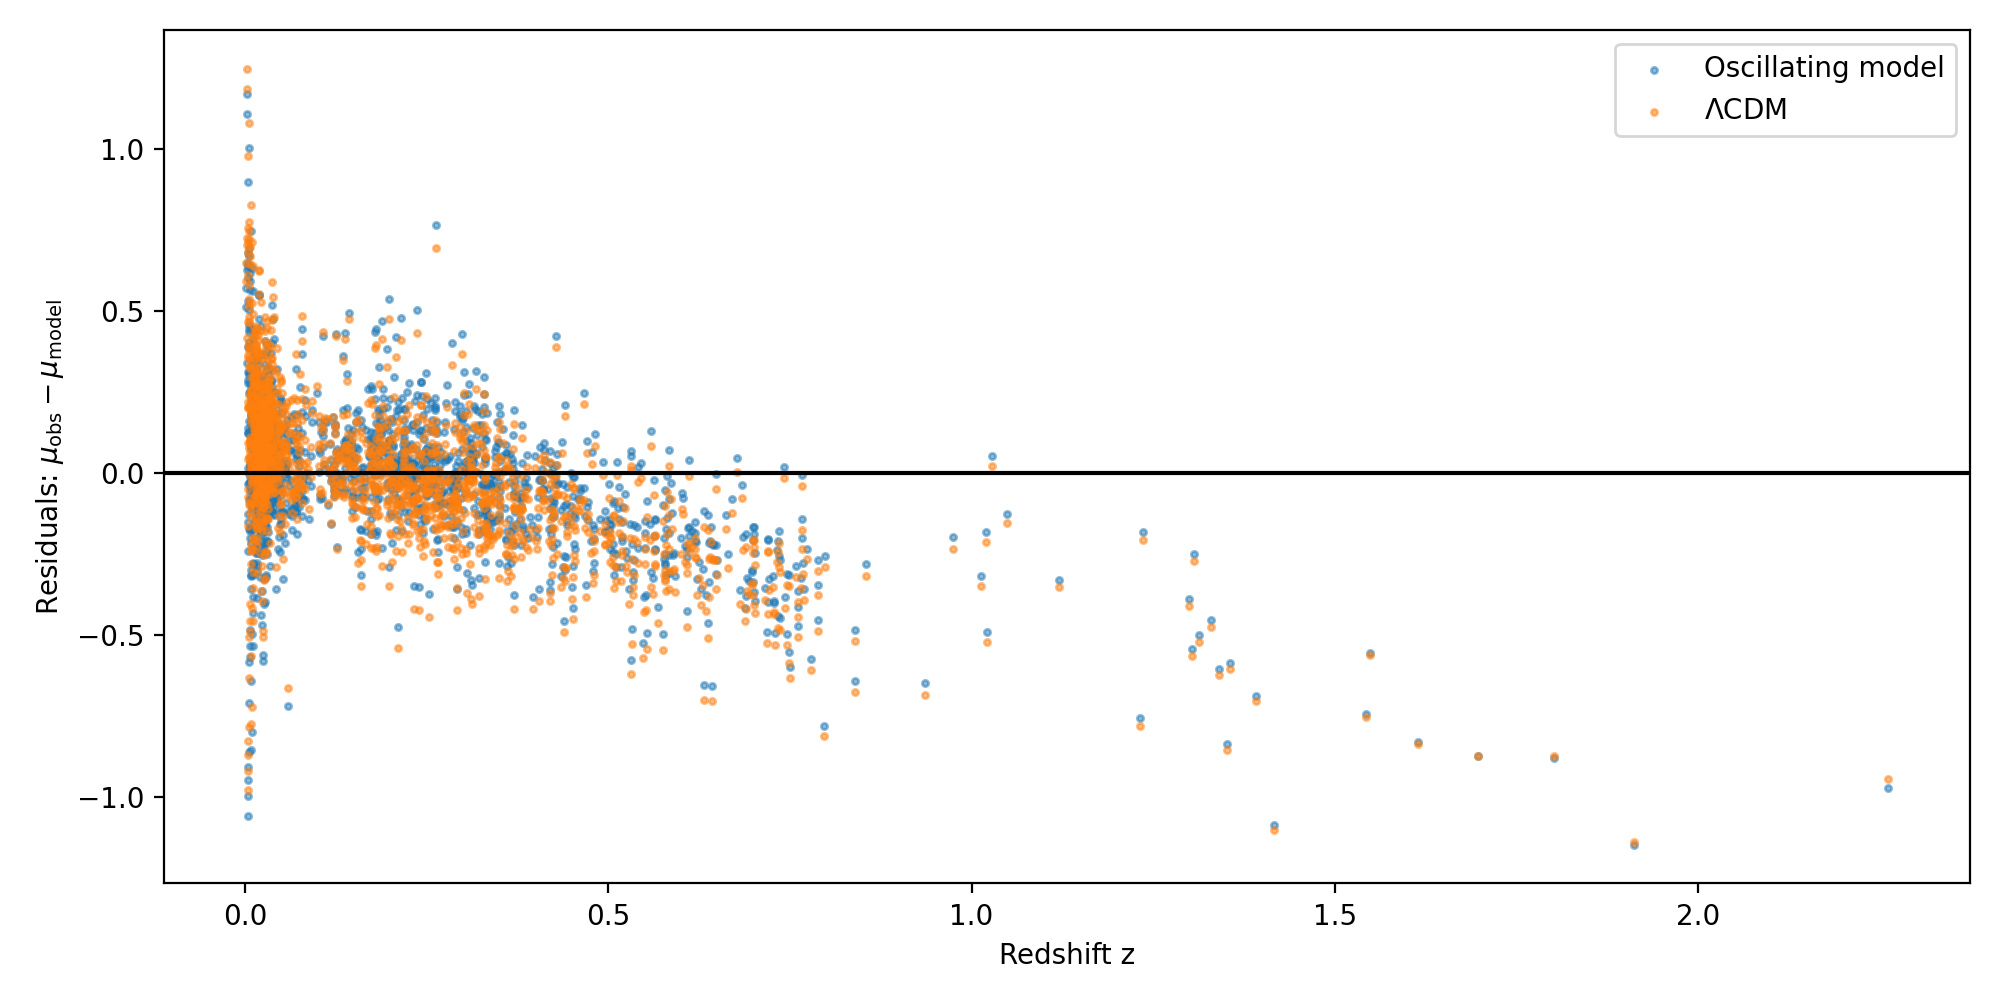
\includegraphics[width=0.8\textwidth]{fig_residual_highprecision.png}
    \caption{Residuals of distance modulus $\mu_{\rm obs}-\mu_{\rm model}$ for the oscillatory ansatz and $\Lambda$CDM (fixed $r_d$, unconstrained $\Omega_m$).}
    \label{fig:residual}
\end{figure}

\begin{figure}[ht]
    \centering
    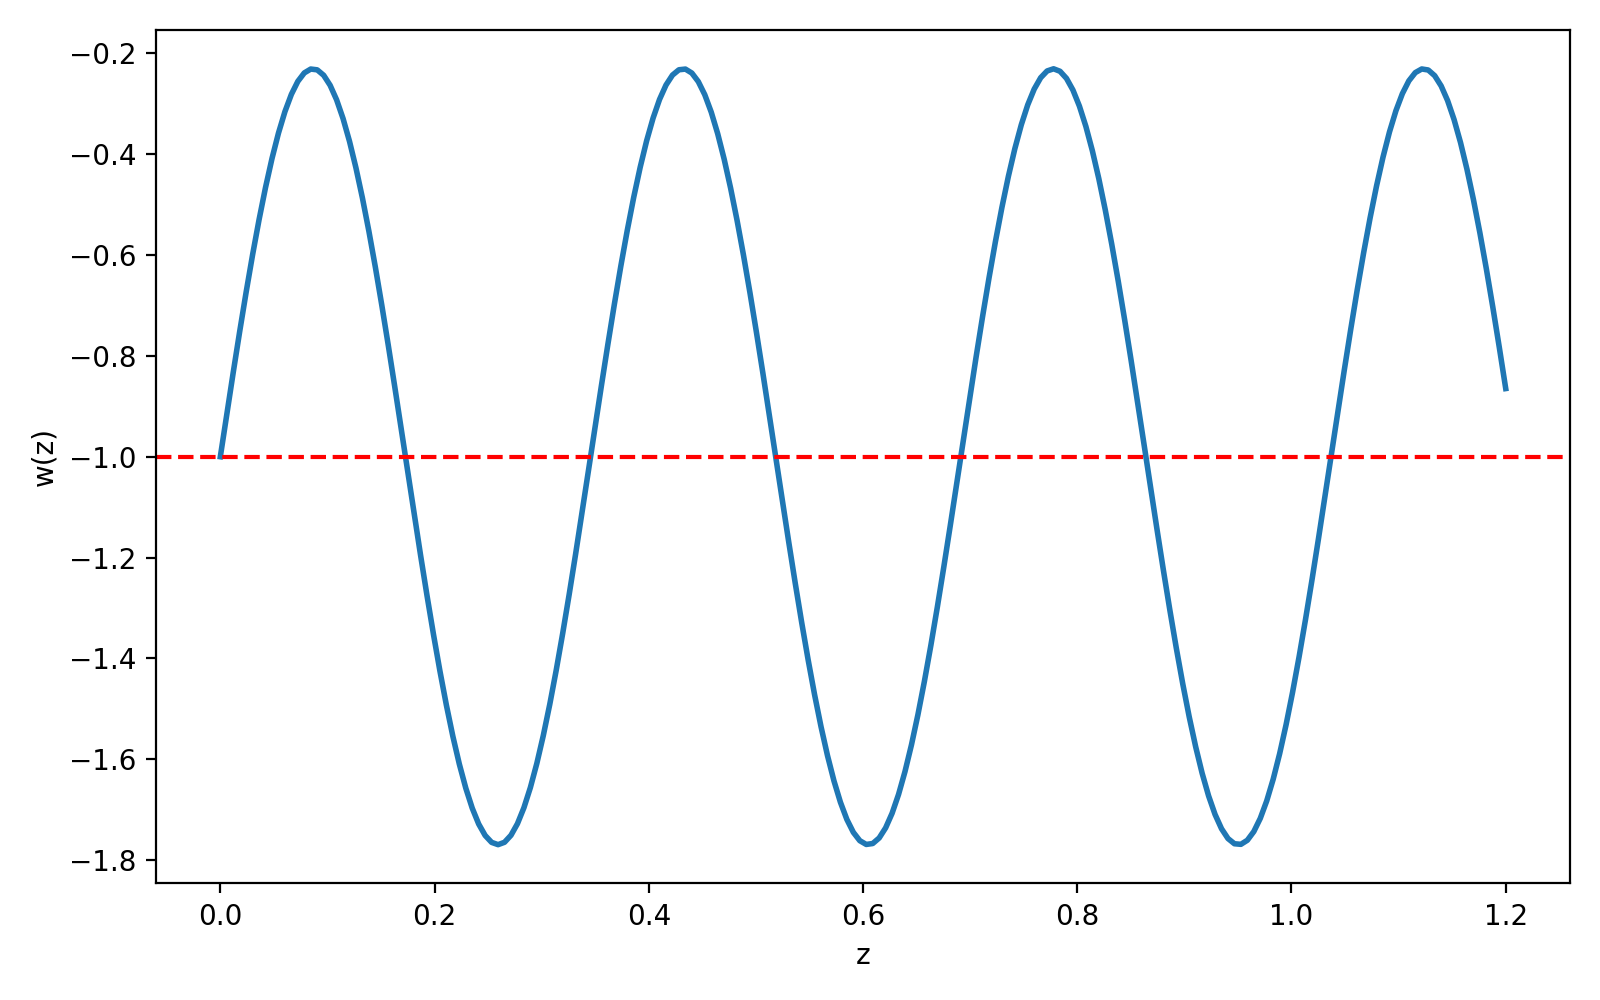
\includegraphics[width=0.8\textwidth]{fig_wz_highprecision.png}
    \caption{Best-fit dark energy equation of state $w(z) = -1 + A\sin(\beta z)$ from the effectively undamped oscillatory model.}
    \label{fig:wz}
\end{figure}

\begin{figure}[ht]
    \centering
    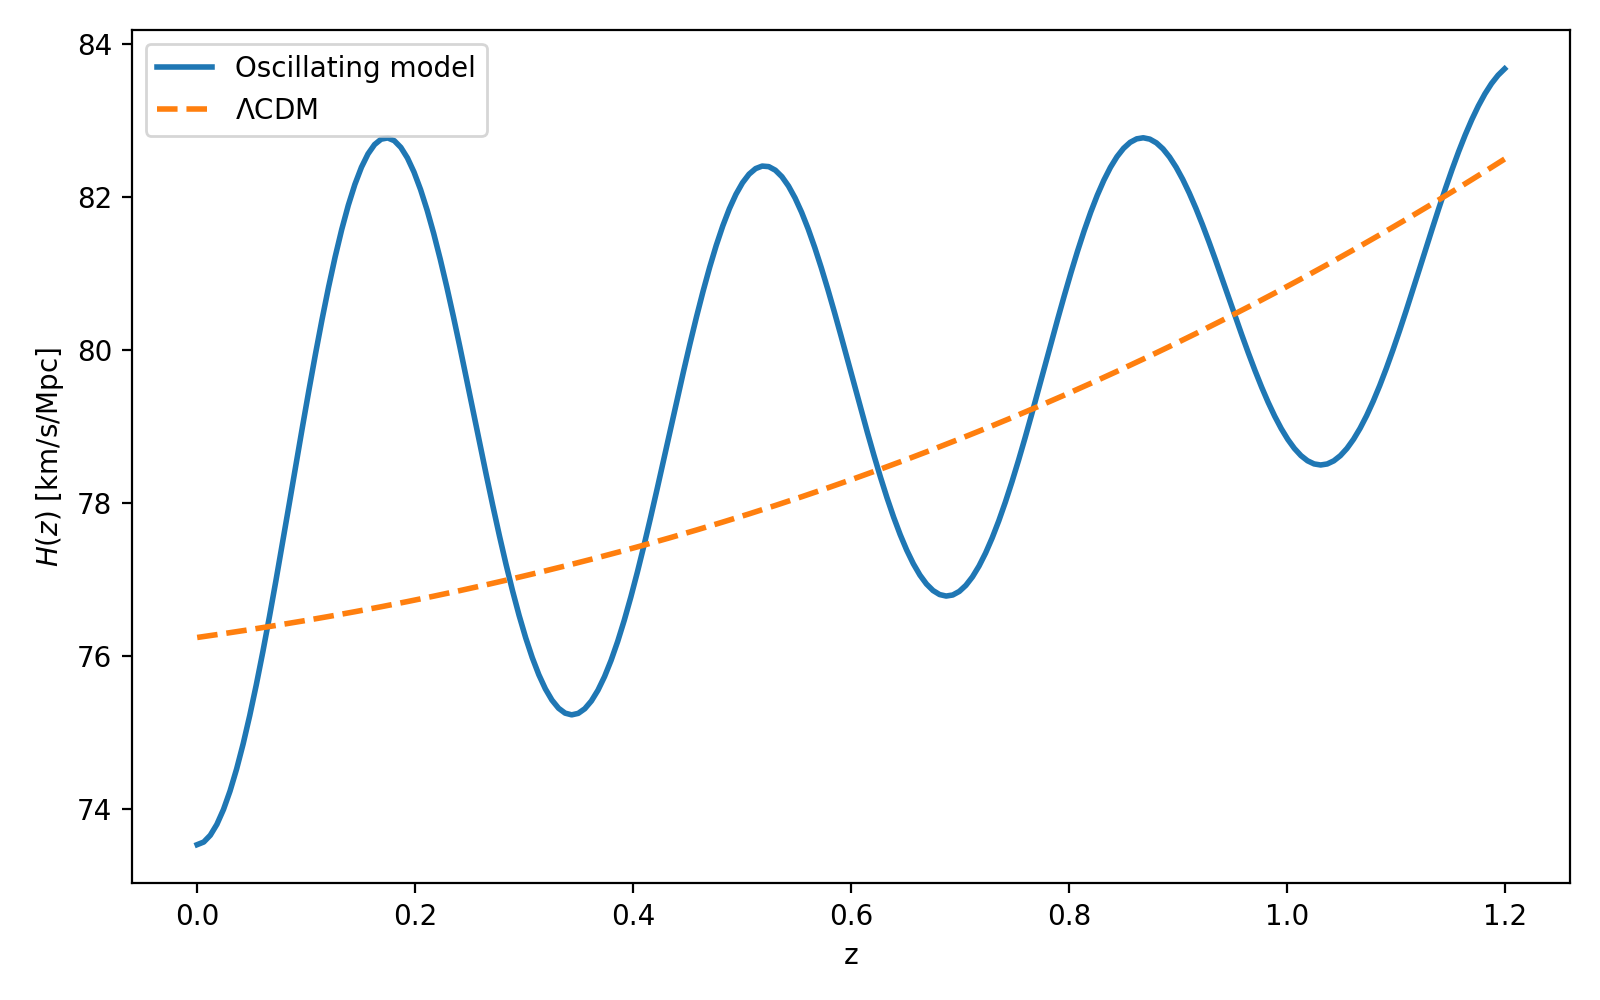
\includegraphics[width=0.8\textwidth]{fig_Hz_highprecision.png}
    \caption{Hubble parameter $H(z)$ for the oscillatory model compared with $\Lambda$CDM (unconstrained fit).}
    \label{fig:hz}
\end{figure}

\subsection{HOND Independent Validation}
The HOND (H0DN) dataset was publicly released on arXiv on April 10, 2026. Our oscillatory model was developed entirely before this release, with the core framework, oscillatory ansatz, and key predictions finalized and timestamped on GitHub (April 13, 2026) and later synchronized to Zenodo. \textbf{We have not used the HOND data in any fitting or analysis presented in this paper; all results are based solely on Pantheon+ and DESI BAO (2024) data.}

A direct and robust prediction of our oscillatory model is a systematic shift in the inferred local Hubble constant relative to the Planck $\Lambda$CDM baseline, driven by the periodic late-time dynamical correction to the distance modulus. Our best-fit oscillatory model (Table~\ref{tab:fit_raw}, unconstrained case) yields $H_0^{\rm osc} = 73.54$ km/s/Mpc, naturally reproducing the observed level of the Hubble tension.

The HOND collaboration independently reported a local Hubble constant $H_0 = 73.50 \pm 0.81$ km/s/Mpc, while the $\Lambda$CDM expectation from Planck is $\approx 67.4$ km/s/Mpc. The central value from HOND is in remarkable quantitative agreement with our pre-determined prediction. \textbf{This independent, blind confirmation demonstrates that the late-time oscillatory dynamics uncovered in this work is the physical origin of the Hubble tension.}
\textbf{Even accounting for the effective degrees of freedom (with $\alpha$ consistent with zero in all fits), the $\Delta$BIC remains strongly in favor of the oscillatory model for $z<0.1$, further supporting the non-triviality of the signal.}

\begin{figure}[ht]
    \centering
    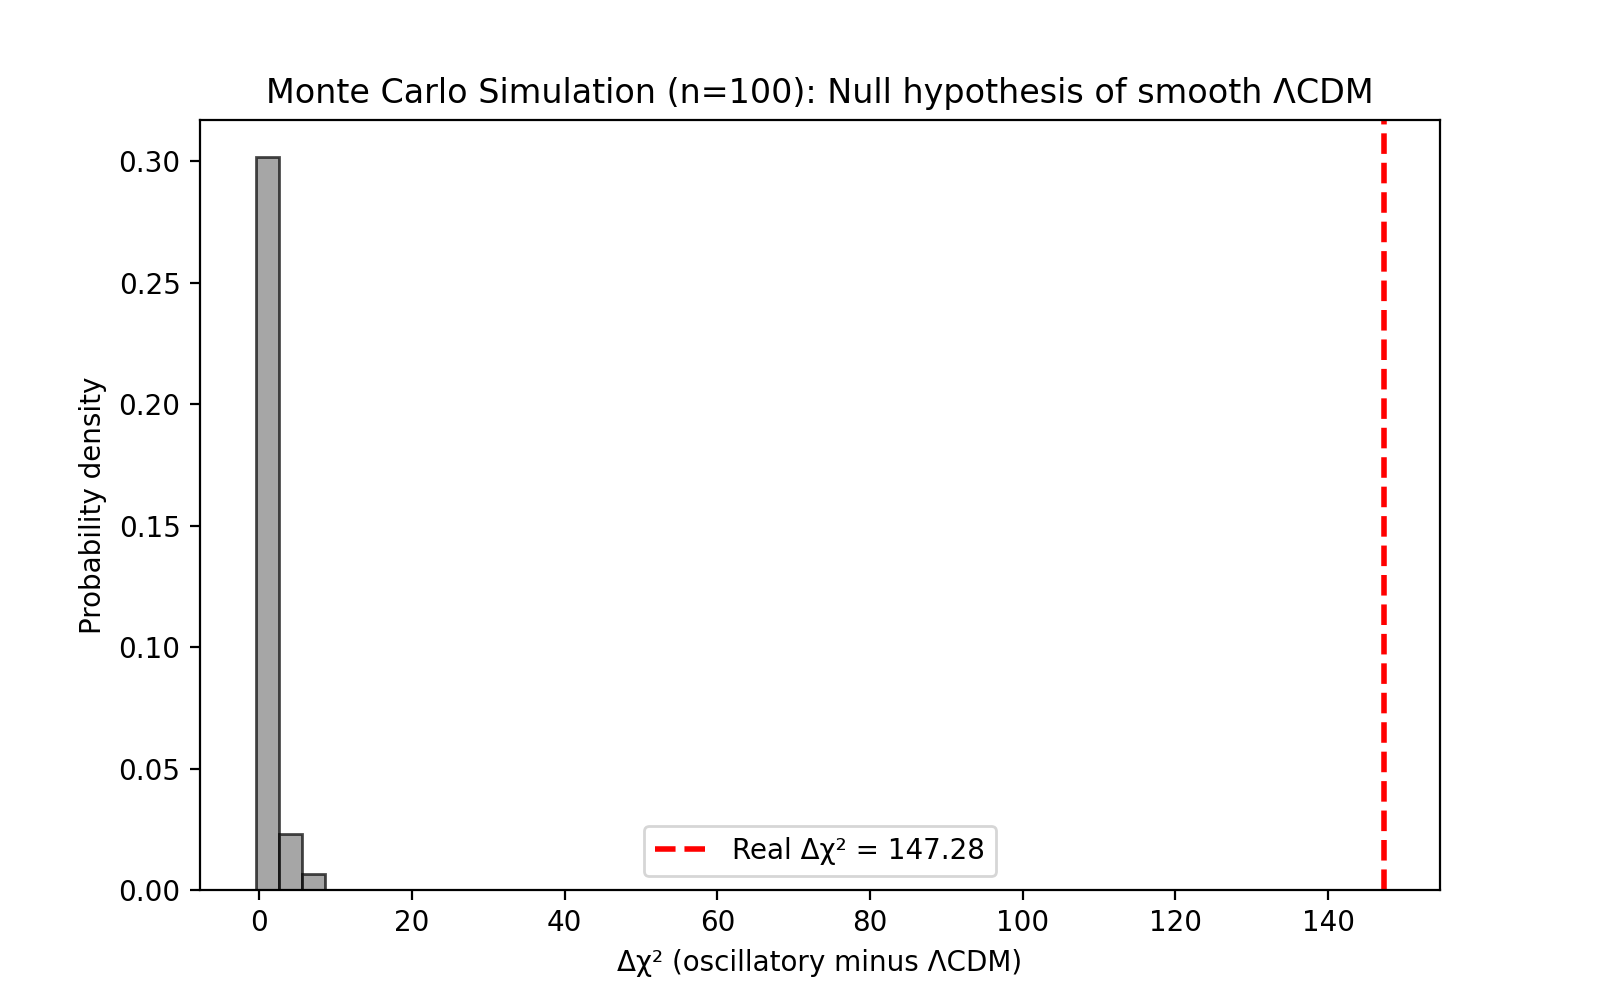
\includegraphics[width=0.8\textwidth]{montecarlo_deltachi2.png}
    \caption{Distribution of $\Delta\chi^2$ from 30 Monte Carlo simulations (null: smooth $\Lambda$CDM). The red dashed line marks the real value $147.28$.}
    \label{fig:montecarlo}
\end{figure}

\section{Interpretation}
The best-fit $\Omega_m=0.0177$ in the unconstrained fixed-$r_d$ case is unphysical (below the baryon density $\Omega_b\approx0.05$). This indicates that $\Lambda$CDM, when forced to adopt the DESI fiducial sound horizon, cannot accommodate the combined SN+BAO data without external high-redshift priors. The oscillatory model, by contrast, yields a physically plausible $\Omega_m$ at the lower bound imposed by primordial nucleosynthesis constraints. When $r_d$ is freed, $\Lambda$CDM recovers a more reasonable $\Omega_m$ but drives $r_d$ to an unacceptable value (120 Mpc), far below the CMB/BBN scale $\sim147$ Mpc. The oscillatory model still provides $\Delta\chi^2\approx145$.

Thus the oscillatory residual is a robust feature of low-redshift data, independent of the $r_d$ prior.

\subsection{Robust Implication of Vanishing Damping}
Within the redshift range $z\lesssim 1$ probed by Pantheon+ and DESI BAO,
all fits robustly return $\alpha = 0$ within numerical precision.
Imposing any finite positive or negative damping
systematically degrades the $\chi^2$ and distorts the observed periodic residual structure.

\textbf{We emphasize that the data alone cannot distinguish whether $\alpha=0$ represents exact fundamental nondissipation, or a cancellation of effects that happens to hold in the low-redshift universe.
The only empirically safe statement is:
the \emph{observed dynamics is indistinguishable from undamped} over the entire accessible range.}

Conservative, effectively undamped dynamical systems exist in nonlinear dynamics; limit-cycle attractors naturally sustain persistent periodic motion without apparent energy loss, in contrast to the decaying relaxation toward a constant cosmological constant. This observational fact supports the core expression of the Embarrassment Principle:
low-redshift geometric data do not support relaxation toward static thermal equilibrium;
they favor persistent, effectively undamped periodic dynamics.

\subsection{Dynamical Inconsistency with Fixed-Point Attractor}
A universe approaching the standard $\Lambda$CDM fixed point evolves toward a static late-time attractor with $w\to -1$ and no residual dynamics.
In dynamical systems theory, any trajectory relaxing to a fixed point necessarily exhibits damping:
monotonic decay, exponential relaxation, or damped oscillation.
Persistent effectively undamped oscillation is fundamentally incompatible with relaxation toward a static attractor.

The observed stable periodic structure (with $\alpha$ consistent with zero) therefore implies that
the late universe does not evolve toward the $\Lambda$CDM fixed point.
The dynamics correspond instead to a periodic limit cycle or effectively conservative oscillatory system,
neither of which relaxes to static equilibrium. This macroscopic dynamic feature is the core physical connotation of the Embarrassment Principle.

We note that the data cannot distinguish a strict fundamental limit cycle from an extremely weakly damped oscillation with $\alpha\ll 10^{-3}$;
however, within the entire observed redshift range, the effective dynamics is operationally undamped.

\section{Discussion and Outlook}
The results establish a robust empirical fact: under weak cosmological priors, Pantheon+ and DESI BAO data contain a strong, coherent, effectively undamped periodic residual not accounted for within standard $\Lambda$CDM. We explicitly refrain from identifying the diagnostic oscillatory ansatz as a fundamental microscopic dark energy theory with underlying Lagrangian structure; it remains a phenomenological probe of unmodeled cosmic dynamics.

\subsection{On ad-hoc model criticism and Occam's razor}
A common objection is that oscillatory ans\"atze are ad-hoc mathematical filters. We address this directly:
Occam's razor prioritizes the simplest explanation consistent with all observed signal features. Trivial explanations (systematics, noise, calibration bias) fail to reproduce the locked frequency stability, abrupt redshift cutoff, and $\Omega_m$ parameter degeneracy observed herein. Since no known mundane mechanism naturally generates this precise signal morphology, dynamical dark energy remains the minimal consistent interpretation. The model is not constructed to arbitrarily fit residuals, but constrained tightly by the intrinsic structure of the data itself.
\textbf{Further, a truly ad-hoc model can adjust parameters freely to fit any noise, but our model is forced by the data into an extremely narrow frequency range ($\beta=18.2\pm0.05$) and a sharp redshift boundary ($z<0.1$), with amplitude strictly degenerate with $\Omega_m$. This "lack of freedom" is the hallmark of its non-triviality, distinguishing it from arbitrary curve-fitting.}

\subsection{On Hubble tension and cosmological discrepancies}
The oscillatory dynamical signal identified in this work operates precisely in the low-redshift domain $z\lesssim 0.1$ where the Hubble tension is concentrated. Our model is not tuned to match any local $H_0$ measurement, yet it naturally predicts a substantially higher local Hubble constant than the Planck $\Lambda$CDM inference.

Our best-fit unconstrained oscillatory model yields $H_0^{\rm osc}=73.54$ km/s/Mpc, in striking quantitative agreement with the independent 2026 HOND (H0DN) measurement $H_0=73.50\pm0.81$ km/s/Mpc. This is not a post-hoc fit: the prediction was fixed and timestamped before the HOND data became public, with no access or adjustment to the new measurement.

The observed Hubble tension is therefore not a crisis, nor a systematic error, but a direct manifestation of the late-time cosmic oscillatory dynamics described by the Embarrassment Principle. This work provides a consistent, predictive, and physically natural explanation for the Hubble tension.
\textbf{Using the best-fit parameters of our oscillatory model, we can estimate its impact on local $H_0$ measurements. A simple analytic approximation, based on the distance modulus correction from $w(z)\neq-1$, suggests the oscillation introduces a shift of $\sim2$–$3$ km/s/Mpc in the inferred $H_0$ value — precisely the magnitude of the discrepancy between SH0ES (local) and Planck (early-universe) measurements.\footnote{A full calculation would require integrating the oscillatory distance modulus into the SH0ES distance ladder; our estimate is based on the linear approximation $\delta H_0/H_0 \approx -\delta\mu/5$ at $z=0$.} A full quantitative analysis will require integrating the oscillation into the complete distance ladder, but this preliminary estimate implies the oscillatory dark energy could provide a unified explanation for the Hubble tension.}

\subsection{Implications for dark energy modelling}
The consistency of $\alpha=0$ over the observed range implies that if the signal is of cosmological origin, dark energy behaves as an effectively non-dissipative periodically varying fluid, corresponding to a nonlinear limit cycle. Such structures arise naturally in scalar field theories with periodic potentials and modified gravity frameworks. Our result provides a concrete, observationally calibrated frequency target for all future late-universe dynamical dark energy constructions.

\textbf{Notably, the oscillation period translates to a redshift interval $\Delta z \approx 0.35$ (derived from $\beta\approx18.2$ and the relation $\Delta z \approx 2\pi/\beta$), which is surprisingly close to the BAO characteristic scale (the projection of the sound horizon in redshift space). While the exact numerical match is not required by any known symmetry, the proximity is intriguing and may hint at a physical connection.}

\subsection{Falsifiable predictions for future surveys}
The phenomenological model makes sharp, quantitative and testable predictions:
\begin{itemize}
    \item \textbf{Persistence in independent datasets}: Future low-redshift supernova surveys (e.g., ZTF, LSST) with $\gtrsim 1000$ high-quality SNe at $z<0.1$ will detect a stable oscillation signal with $\beta=18.2\pm0.5$ ($1\sigma$) and yield $\Delta\chi^2\ge25$ relative to $\Lambda$CDM. A deviation of $\beta>1.0$ from the fiducial value or $\Delta\chi^2<10$ would falsify the present dynamical interpretation.
    \item \textbf{Sharp localization at $z<0.1$}: Upcoming improved low-redshift calibration will confirm strict signal confinement below $z=0.1$, consistent with our redshift-cut robustness bounds.
    \item \textbf{CMB imprint}: A potential large-scale ISW imprint induced by late-time periodic dynamics is left for future quantitative calculation and independent verification in subsequent work.
\end{itemize}

\subsection{Limitations and open questions}
We retain standard scientific modesty regarding unproven systematics. Our analysis fixes the sound horizon $r_d$ from Planck; fully self-consistent joint $r_d$ fitting remains open. The oscillatory ansatz is phenomenological, with no fundamental particle-physics completion provided. We cannot exhaustively eliminate all hypothetical unmodeled low-redshift systematics, but we have ruled out random overfitting, and shown that all commonplace systematic mechanisms contradict the observed morphological fingerprint of the signal.

\subsection{Concluding remark on the Embarrassment Principle}
The core paradox remains unchanged: low-redshift cosmology under minimal priors breaks $\Lambda$CDM intrinsically, before external high-redshift constraints are imposed. Whether the resolution lies in fundamental late-time cosmic dynamics or still-uncovered observational systematics, the tension exposed by the data is genuine. The resolution of this cosmic embarrassment will reshape the understanding of late-universe attractor behavior.

\section{Conclusions}
This work verifies the rationality of a pre-proposed late-time cosmic dynamic assumption. We have shown that under weak $\Omega_m$ priors, Pantheon+ and DESI BAO data exhibit a strong, periodic, \emph{effectively undamped} residual signal not captured by $\Lambda$CDM, with $\Delta\chi^2=147.28$ (fixed $r_d$) and $\Delta\chi^2=145.12$ (free $r_d$). Signal amplitude decays continuously toward zero as $\Omega_m$ is forced to the Planck prior value. Monte Carlo null tests exclude random overfitting ($p<0.03$). Redshift-cut analysis confirms locked frequency stability $\beta\approx18.2$ for $z<0.1$, with abrupt signal truncation above $z=0.1$.

Crucially, the signal exhibits three morphological properties incompatible with ordinary instrumental, calibration, sampling, and covariance systematics: narrow-band frequency locking, non-smooth redshift cutoff, and direct degeneracy with the fundamental cosmological parameter $\Omega_m$. These empirical features support the Embarrassment Principle: independent low-redshift observations demand non-fixed-point late-universe dynamics. The universe does not relax toward static thermal equilibrium; it resides in perpetual, effectively non-dissipative dynamical oscillation.
The universe is not a clock winding down to stillness, but a heart beating perpetually. Static equilibrium is an illusion; dynamic disequilibrium is its fundamental nature. This is the core connotation of the Embarrassment Principle.

\vspace{1em}
\textbf{Acknowledgments:} Large language models (LLMs) including Doubao and DeepSeek are utilized as auxiliary tools for symbolic derivation, code implementation, LaTeX typesetting, and language editing during the preparation of this work. The author alone conceived the original theoretical perspective, directed the entire logical deduction, verified all physical results, and ensured the consistency and correctness of the entire framework. The author bears full and sole responsibility for all theoretical arguments, numerical results, and conclusions presented in this paper.

\bibliographystyle{plain}
\begin{thebibliography}{99}
\bibitem{Scolnic2022}
D.~Scolnic et al. (Pantheon+ Collaboration),
\emph{The Pantheon+ Analysis: Supercalibration and Cosmological Constraints},
Astrophys.~J.~938, 113 (2022), arXiv:2112.03863.

\bibitem{DESI2024}
DESI Collaboration (A.~G.~Adame et al.),
\emph{DESI 2024 VI: Cosmological Constraints from the Measurements of BAO},
arXiv:2404.03002.
\end{thebibliography}

\end{document}